\documentclass[12pt, letterpaper]{article}
\usepackage[left=1.00in, right=1.00in, top=1.00in, bottom=1.00in]{geometry}
\usepackage{amsmath}
\usepackage{apacite}
\usepackage{graphicx}

\title{Chapter 2}
\author{Daniel C. Furr}
\date{\today}


\begin{document}

\newcommand{\genupsilonsq}{0.11}
\newcommand{\gentau}{\{0.00, 0.10, 0.30, 0.50\}}
\newcommand{\gentausq}{\{0.00, 0.01, 0.09, 0.25\}}
\newcommand{\genrsq}{\{1.00, 0.92, 0.55, 0.30\}}

\newcommand{\comment}[1]{{\footnotesize[\textit{#1}]}}

\maketitle

\tableofcontents
\newpage
{\footnotesize }


\section{Introduction}

%\begin{enumerate}
%	\item Conducting holdout cross-validation require a decision of what parts of model are exchangeable. Approximations also depend on this, though may not be obvious. Easy for non-clustered data. For clustered data, must decide whether clusters are exchangeable. In a model with likelihood that is marginal over clusters, it is implied that clusters are exchangeable.
%	\item Item response models generally have fixed part for items and random part for persons, reflecting an expectation that new data would have new people responding to the original items. CV ``over persons'' may be used to select person predictors.
%	\item Not appropriate for selecting predictors for item difficulty. Need CV ``over items''. LLTM marginal likelihood not appropriate. LLTME marginal likelihood is appropriate, though difficult.
%	\item This paper shows...
%\end{enumerate}

The use of cross-validation with clustered data requires a decision as to what aspects of the data are exchangeable, and so are resampled in new data, and what aspects persist. For item response data, in which responses are nested both within persons and items simultaneously, new data may consist of a new group of persons responding to the original items, which will be referred to as cross-validation ``over persons.'' Alternatively, new item response data may entail a new set of items presented to the original group of persons, which will be referred to as cross-validation ``over items.'' Other variations are possible, such as new data from both the same persons and items, an exact replication of the original data collection, or new data from both new persons and items.

The form of new data determines what inferences may be made using cross-validation. For example, cross-validation must be done over persons in order to select for person ability predictors in a latent regression Rasch model \cite{}. In other words, a new sample of persons are needed to assess the predictors for ability. Likewise, if the goal is to choose predictors for item difficulty in a linear logistic test model (LLTM) \cite{}, cross-validation must be performed over items.

The choice of model has strong implications regarding which aspects of the data are considered exchangeable, and hence would be resampled in cross-validation, and which are persistent. Specifically, the ``random effects'' are exchangeable, and the ``fixed effects'' are persistent. In general for item response models, person abilities (or their residuals) are modeled as random effects, while items are treated as fixed, implying that a repeat of the data collection would involve a new sample of persons responding to the same items.

In this chapter, the difference in efficacy of employing cross-validation over persons versus over items with LLTM is investigated. AIC, a single dataset approximation to cross-validation, is shown to correspond to cross-validation over persons, which is not effective for the selection of item predictors.


\section{Simulation and analysis methods}

\subsection{Data generation}

%Data are simulated for varying numbers of persons ($P$) and items ($I$) using the model described in Chapter~1. 
Data are simulated using the model described in Chapter~1. 
Specifically, the composite item difficulties are generated as
\begin{equation}
	\delta_i = x_{1i}\beta_1 + x_{2i}\beta_2 + x_{3i}\beta_3 + x_{4i}\beta_4 + x_{2i}x_{3i}\beta_5 + \epsilon_i
\end{equation}
\begin{equation}
	\epsilon_i \sim \mathrm{N}(0, \tau^2)
,\end{equation}
where $x_{1i} = 1$ is an intercept and $x_{2i}$, $x_{3i}$, and $x_{4i}$ are indicator variables which each equal 1 for half of the items and 0 for the remainder. Each possible combination of the indicators occurs an equal number of times, and the generating model includes one interaction, $x_{2i}x_{3i}$. Table~\ref{tab:X} provides the design matrix for item covariates. The rows of the design matrix are repeated to accommodate multiples of $I = 8n_p$.

% matrix: X file: figs/table_x.tex  23 Oct 2015 12:20:52
\begin{table}[htbp]
\caption{\label{tab:X} Items design matrix}\centering\medskip
\begin{tabular}{ccccc} \hline \hline
$x_1$ & $x_2$  & $x_3$  & $x_4$  \\  \hline 
1 & 0 & 0 & 0 \\  
1 & 0 & 0 & 1 \\  
1 & 0 & 1 & 0 \\  
1 & 0 & 1 & 1 \\  
1 & 1 & 0 & 0 \\  
1 & 1 & 0 & 1 \\  
1 & 1 & 1 & 0 \\  
1 & 1 & 1 & 1 \\  
\hline \hline \end{tabular}
\end{table}


The composite abilities are generated as
\begin{equation} \label{eq:theta}
	\theta_p = w_{1p}\gamma_1 + w_{2p}\gamma_2  + \zeta_p
\end{equation}
\begin{equation} \label{eq:zeta}
	\zeta_p \sim \mathrm{N}(0, \sigma^2)
,\end{equation}
where $w_{1p}$ and $w_{2p}$ are also crossed indicator variables. Table~\ref{tab:W} presents the design matrix for person covariates, the rows of which are repeated to accommodate the $P = 4n_i$ persons.

% matrix: W file: figs/table_w.tex  23 Oct 2015 12:20:52
\begin{table}[htbp]
\caption{\label{tab:W} Persons design matrix}\centering\medskip
\begin{tabular}{cc} \hline \hline
$w_1$  & $w_2$  \\  \hline 
0 & 0 \\  
0 & 1 \\  
1 & 0 \\  
1 & 1 \\  
\hline \hline \end{tabular}
\end{table}


A key feature of the generated datasets (and data of this type more generally) is the extent to which the item covariates account for the composite item difficulties. To this end, let $\upsilon^2 = \mathrm{var}(x'\mathbf{\beta})$ represent the variance of the structural part of item difficulty. Because of the item design, $\upsilon^2$ does not vary between simulated datasets, even if they have differing numbers of items (in multiples of eight). The total item variance is $\upsilon^2 + \tau^2$. Then
\begin{equation}
R^2 = \frac{\upsilon^2}{\upsilon^2 + \tau^2}
\end{equation}
represents the proportion of item variance accounted for by the item predictors. 

The generating values for the structural part of item difficulties are $\beta = \{ -.5, .5, .5, .5, -.5 \}$ in all simulation conditions, and so $\upsilon^2 = \genupsilonsq$. Figure~\ref{fig:rsq-vs-tau} displays $R^2$ as a function of $\tau$ with $\upsilon^2$ fixed to this value. The points indicate the generating values of $\tau$, which are $\tau \in \{\gentau\}$ (or equivalently,  $\tau^2 \in \{\gentausq\}$). These values yield $R^2 \in \{\rsq\}$. On the person side, the generating values are fixed across conditions, with $\gamma = \{ .5, .5 \}$ and $\sigma = 1$. 
%The numbers of persons and items vary: $I \in \{32, 128\}$ and $P \in \{300, 1000\}$.

\begin{figure}[tbp]
	\centering
	\includegraphics{chapter_2/figs/rsq_vs_tau.pdf}
	\caption{Proportion of total item variance explained by the item covariates ($R^2$) versus residual item standard deviation ($\tau$) in the simulated datasets. The points indicate generating values of $\tau \in \{\gentau\}$.}
	\label{fig:rsq-vs-tau}
\end{figure}

%In summary, three factors are varied between simulation conditions in a crossed design: $\tau$ (and by extention, $R^2$), $I$, and $P$. 
%All other elements are fixed across conditions. 
In summary, the same generating values and design matrices are used across all simulation conditions.
In the first simulation, generating values of $\tau$ are varied. In the second, the number of items are varied.
To employ cross-validation, multiple datasets are simulated within each replication: the ``test'' dataset, a ``training'' dataset representing a sample with new items (corresponding to new draws of $\epsilon_i$), and another training dataset representing a sample with new persons (new draws of $\zeta_p$).


\subsection{Models}

Three models, differing only in specification of $\delta_i$, are fit. Model 1 includes only the ``main effects'' for the item covariates:
\begin{equation}
\delta_i^{(1)} = x_{1i}\beta_1 + x_{2i}\beta_2 + x_{3i}\beta_3 + x_{4i}\beta_4
.\end{equation}
Model 2 adds an interaction:
\begin{equation}
\delta_i^{(2)} = x_{1i}\beta_1 + x_{2i}\beta_2 + x_{3i}\beta_3 + x_{4i}\beta_4
+ x_{2i}x_{3i}\beta_5
.\end{equation}
Model 3 adds an additional, extraneous interaction:
\begin{equation}
\delta_i^{(3)} = x_{1i}\beta_1 + x_{2i}\beta_2 + x_{3i}\beta_3 + x_{4i}\beta_4
+ x_{2i}x_{3i}\beta_5 + x_{3i}x_{4i}\beta_6
.\end{equation}
Each analysis model models ability as in Equations~\ref{eq:theta} and \ref{eq:zeta} while omitting the item residual $\epsilon_i$. 
Model~2 has the correct fixed part of the model, and consequently Model~2 matches the data generating model when $\tau = 0$. Otherwise, none of three match the data generating model.
 
The analysis models are naive, given that in most simulation conditions $\tau > 0$. 
More generally, the item predictors in an LLTM are not expected to exactly fit the item difficulties in actual application.
Omitting item residuals is overly restrictive and results in failure to model the within-item dependency of responses. 
This problem is the same as that which arises from fitting a non-hierarchical model to clustered data. 
However, fitting random effects for both person and items is prohibitively difficult with maximum likelihood estimation, so researchers often resort to fitting models like the above.


\section{Simulation~1}

Datasets consisting of $\npersons$ persons and $\nitems$ items are generated with values of $\tau \in \gentau$. The simulation is carried out for $\nreps$ replications for each value of $\tau$. 


\subsection{Naive cross-validation methods}

One naive approach to model selection is the use of significance testing for parameters. In order to select among nested analysis models, a researcher may conduct likelihood ratio tests on pairs of models. If the test rejects the simpler model in a pair, the more complex model is retained and compared against a still more complex model. This procedure continues until the test fails to reject a model or when only the most complex model remains.

The first panel of Figure~\ref{fig:select-overtau} provides the proportion of times each model is selected using likelihood ratio tests in the simulation.
Model~2 is selected the large majority of times when $\tau$ is zero or small, corresponding to situations in which this model is the true model or almost so.
As $\tau$ becomes greater, the more complex Model~3 is selected increasingly often.
The same results would be expected if Wald tests on the interaction terms were used for selection instead of likelihood ratio tests.

%Adding item residuals $\epsilon_i$ to the analysis models would provide correct standard errors and p-values. Such a model is prohibitively difficult to fit without resorting to Monte Carlo methods, though. 
An appealing alternative is AIC, defined as
\begin{equation} \label{eq:aic}
\mathrm{AIC} = \mathrm{dev_{in}} + 2k_\mathrm{AIC}
,\end{equation}
where $k_\mathrm{AIC}$ is the number of model parameters. The model with the lowest value of AIC is selected.
AIC is suitable both for comparing non-nested models, which likelihood ratio tests cannot do, and for comparing many models simultaneously, which bring up problems of multiple hypothesis for likelihood ratio tests. Further, AIC explicitly frames model selection as a trade off between model fit and complexity. \comment{Explain further, including  Kullback–-Leibler divergence.}
The results of using AIC with the simulated datasets are presented in Figure~\ref{fig:select-overtau}. 
%These results follow similar patterns as for selection by p-values, though a bit worse.

\begin{figure}[tbp]
	\centering
	\includegraphics{chapter_2/figs/select_overtau.pdf}
	\caption{Proportion of times each model was selected across differing generating values for residual item standard deviation ($\tau$), shown for differing selection methods. Each simulation condition was replicated $\nreps$ times with datasets consisting of $\npersons$ persons and $\nitems$ items. Model~2 is the true model when $\tau = 0$.}
	\label{fig:select-overtau}
\end{figure}

AIC is an approximation for holdout cross-validation, in which a model is estimated using a ``training'' dataset and then evaluated on a ``test'' dataset \comment{show Kullback-–Leibler divergence formula}. Specifically,
\begin{equation}
	k_\mathrm{AIC} \approx k_\mathrm{CV} = \frac{\mathrm{dev_{out}} - \mathrm{dev_{in}}}{2}
,\end{equation}
where $\mathrm{dev_{in}}$ is the deviance of the fitted model in the training data, and $\mathrm{dev_{out}}$ is the deviance of the model in the test data given parameter estimates obtained from the training data. 
\comment{Equation is vague. Is it for one application of CV, or a long run quantity.}
For the LLTM, $k_\mathrm{AIC}$ approximates the $k_\mathrm{CV}$ that results from test data consisting of a new sample of persons responding to the same items, or in other words, cross-validation over persons. \comment{Explain why, from chapter 1 or cite papers.} 
%$2k$ in Equation~\ref{eq:aic} may be viewed as an adjustment to the deviance of the model fit to the training data owing to uncertainty in the parameter estimates. 

The correct values for $k_\mathrm{CV}$ from cross-validation over persons may be estimated from the simulation.
This is presented in the left panl of Figure~\ref{fig:k-overtau}. The empirical results regarding $k_\mathrm{CV}$ are similar to those given by AIC (\aic[and]) with some variation across values for $\tau$. Importantly, the difference between models is consistently about one, which agrees with AIC.

\begin{figure}[tbp]
	\centering
	\includegraphics{chapter_2/figs/k_overtau.pdf}
	\caption{Estimated effective number of parameters ($k$) for the models by value of $\tau$, shown for two cross-validation methods. $k$ is the difference between the out-of-sample and in-sample deviance divided by two. AIC relies on an approximation of this quantity, in this case \aic[and], respectively. Each simulation condition was replicated $\nreps$ times with datasets consisting of $\npersons$ persons and $\nitems$ items. Model~2 is the true model when $\tau = 0$.}
	\label{fig:k-overtau}
\end{figure}

In short, AIC performs poorly for model selection in this instance even though it accurately estimates the out-of-sample deviance. Further, cross-validation with new persons also performs poorly, as depicted in Figure~\ref{fig:k-overtau}. Lastly, BIC performs somewhat better but has the same problem. BIC is associated with $k_\mathrm{BIC}$ being \bic[and] for the three models. \comment{Discuss BIC.}


\subsection{Holdout cross-validation for item predictors}

If the focus of model selection is the choice of item predictors, cross-validation schemes based on test data with the same items are wrongheaded. A useful approach instead is to consider how the item predictors will fare for a new set of items constructed with the same item covariates. To this end, the analysis models are fit to a training dataset and then evaluated on a holdout dataset representing the same persons and new items. 

Figure~\ref{fig:select-overtau} provides the proportion of times each model was selected using this scheme. 
Figure~\ref{fig:k-overtau} provides $k_\mathrm{CV}$ under this scheme.
%Across all conditions, Model~2 is selected the majority of times. For $I=32$ items, larger values of $\tau$ are associated with a lower selection proportion for Model~2, while this trend is mitigated when $I=128$.


\section{Simulation~2}

The effect of differing numbers of items are considered.
Datasets consisting of $P = \npersons$ persons and $I \in \{\nitemsoveritems\}$ items are generated with values of $\tau$ fixed at $\gentauoveritems$. The simulation is carried out for $\nreps$ replications for each value of $I$.
Figure~\ref{fig:select-overnitems} shows the proportion of times each model is selected depending on the number of items. Figure~\ref{fig:k-overnitems} provides empirical estimates of the effective number of parameters.

\begin{figure}[tbp]
	\centering
	\includegraphics{chapter_2/figs/select_overnitems.pdf}
	\caption{Proportion of times each model was selected depending on the number of items, shown for differing selection methods. Each simulation condition was replicated $\nreps$ times with datasets consisting of $\npersons$ persons and with $\tau = .3$.}
	\label{fig:select-overnitems}
\end{figure}

\begin{figure}[tbp]
	\centering
	\includegraphics{chapter_2/figs/k_overnitems.pdf}
	\caption{Estimated effective number of parameters ($k$) for the models by number of items, shown for two cross-validation methods. $k$ is the difference between the out-of-sample and in-sample deviance divided by two. AIC relies on an approximation of this quantity, in this case \aic[and], respectively. Each simulation condition was replicated N times with datasets consisting of N persons and with $\tau = .3$}
	\label{fig:k-overnitems}
\end{figure}

\section{Discussion}

\comment{Find papers on choosing between LLTMS. (1) K-fold CV. (2) Consider a linear model to parallel holdout CV with new items. Possible to get marginal likelihood with linear model? (3) Show that AIC works with ``De Boeck'' version of model. (4) Consider extending topic to include linear crossed mixed-effects models.}

%\bibliographystyle{apacite}
%\bibliography{../../Documents/References/references}

\end{document} 






 %%%%%%%%%%%%%%%%%%%%%%%%%%%%%%%%%%%%%%%%%%

\section{Cross-validation with a fixed-persons random-items model.}

A variation on the three models is considered in which the persons are modeled as fixed effects and the items as random effects. The fixed part of the models include the item predictors and and indicator variable for each sum score. Person covariates are omitted. In these ``inverted'' models, the items are regarded as exchangeable rather than the persons. It is posited that AIC for the inverted models would perform correctly for cross-validation inferences that involve new items.

Figure~\ref{fig:k-new-items} provides the estimated effective number of parameters for the models based on the simulations. As may be seen, the values are low in comparison with the count of parameters (\aicitem[and]) and dependent on $\tau$. Figure~\ref{fig:select-aicitem} shows the proportion of times each inverted model was selected using AIC.

\begin{figure}[tbp]
	\centering
	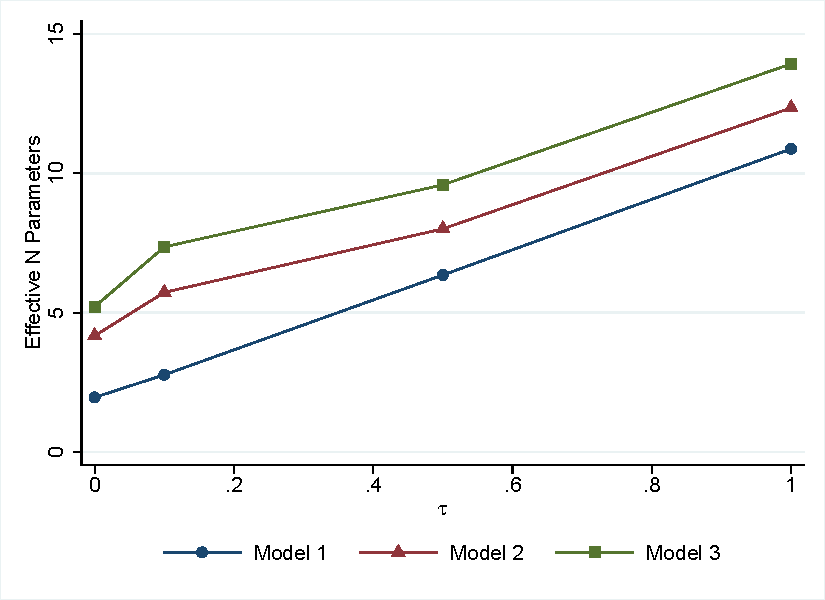
\includegraphics[height=3in, trim = 1mm 1mm 1mm 1mm, clip=true]
	{chapter_2/figs/p_newitems.pdf}
	\caption{Estimated effective number of parameters for models fit to test data consisting of the same persons responding to new items.}
	\label{fig:k-new-items}
\end{figure}

\begin{figure}[tbp]
	\centering
	\includegraphics[height=3.5in, trim = 1mm 1mm 1mm 1mm, clip=true]
	{chapter_2/figs/select_aic2.pdf}
	\caption{Proportion of times each model was selected using AIC with the ``inverted'' models.}
	\label{fig:select-aicitem}
\end{figure}


